% Options for packages loaded elsewhere
\PassOptionsToPackage{unicode}{hyperref}
\PassOptionsToPackage{hyphens}{url}
%
\documentclass[
]{article}
\usepackage{amsmath,amssymb}
\usepackage{iftex}
\ifPDFTeX
  \usepackage[T1]{fontenc}
  \usepackage[utf8]{inputenc}
  \usepackage{textcomp} % provide euro and other symbols
\else % if luatex or xetex
  \usepackage{unicode-math} % this also loads fontspec
  \defaultfontfeatures{Scale=MatchLowercase}
  \defaultfontfeatures[\rmfamily]{Ligatures=TeX,Scale=1}
\fi
\usepackage{lmodern}
\ifPDFTeX\else
  % xetex/luatex font selection
\fi
% Use upquote if available, for straight quotes in verbatim environments
\IfFileExists{upquote.sty}{\usepackage{upquote}}{}
\IfFileExists{microtype.sty}{% use microtype if available
  \usepackage[]{microtype}
  \UseMicrotypeSet[protrusion]{basicmath} % disable protrusion for tt fonts
}{}
\makeatletter
\@ifundefined{KOMAClassName}{% if non-KOMA class
  \IfFileExists{parskip.sty}{%
    \usepackage{parskip}
  }{% else
    \setlength{\parindent}{0pt}
    \setlength{\parskip}{6pt plus 2pt minus 1pt}}
}{% if KOMA class
  \KOMAoptions{parskip=half}}
\makeatother
\usepackage{xcolor}
\usepackage[margin=1in]{geometry}
\usepackage{color}
\usepackage{fancyvrb}
\newcommand{\VerbBar}{|}
\newcommand{\VERB}{\Verb[commandchars=\\\{\}]}
\DefineVerbatimEnvironment{Highlighting}{Verbatim}{commandchars=\\\{\}}
% Add ',fontsize=\small' for more characters per line
\usepackage{framed}
\definecolor{shadecolor}{RGB}{248,248,248}
\newenvironment{Shaded}{\begin{snugshade}}{\end{snugshade}}
\newcommand{\AlertTok}[1]{\textcolor[rgb]{0.94,0.16,0.16}{#1}}
\newcommand{\AnnotationTok}[1]{\textcolor[rgb]{0.56,0.35,0.01}{\textbf{\textit{#1}}}}
\newcommand{\AttributeTok}[1]{\textcolor[rgb]{0.13,0.29,0.53}{#1}}
\newcommand{\BaseNTok}[1]{\textcolor[rgb]{0.00,0.00,0.81}{#1}}
\newcommand{\BuiltInTok}[1]{#1}
\newcommand{\CharTok}[1]{\textcolor[rgb]{0.31,0.60,0.02}{#1}}
\newcommand{\CommentTok}[1]{\textcolor[rgb]{0.56,0.35,0.01}{\textit{#1}}}
\newcommand{\CommentVarTok}[1]{\textcolor[rgb]{0.56,0.35,0.01}{\textbf{\textit{#1}}}}
\newcommand{\ConstantTok}[1]{\textcolor[rgb]{0.56,0.35,0.01}{#1}}
\newcommand{\ControlFlowTok}[1]{\textcolor[rgb]{0.13,0.29,0.53}{\textbf{#1}}}
\newcommand{\DataTypeTok}[1]{\textcolor[rgb]{0.13,0.29,0.53}{#1}}
\newcommand{\DecValTok}[1]{\textcolor[rgb]{0.00,0.00,0.81}{#1}}
\newcommand{\DocumentationTok}[1]{\textcolor[rgb]{0.56,0.35,0.01}{\textbf{\textit{#1}}}}
\newcommand{\ErrorTok}[1]{\textcolor[rgb]{0.64,0.00,0.00}{\textbf{#1}}}
\newcommand{\ExtensionTok}[1]{#1}
\newcommand{\FloatTok}[1]{\textcolor[rgb]{0.00,0.00,0.81}{#1}}
\newcommand{\FunctionTok}[1]{\textcolor[rgb]{0.13,0.29,0.53}{\textbf{#1}}}
\newcommand{\ImportTok}[1]{#1}
\newcommand{\InformationTok}[1]{\textcolor[rgb]{0.56,0.35,0.01}{\textbf{\textit{#1}}}}
\newcommand{\KeywordTok}[1]{\textcolor[rgb]{0.13,0.29,0.53}{\textbf{#1}}}
\newcommand{\NormalTok}[1]{#1}
\newcommand{\OperatorTok}[1]{\textcolor[rgb]{0.81,0.36,0.00}{\textbf{#1}}}
\newcommand{\OtherTok}[1]{\textcolor[rgb]{0.56,0.35,0.01}{#1}}
\newcommand{\PreprocessorTok}[1]{\textcolor[rgb]{0.56,0.35,0.01}{\textit{#1}}}
\newcommand{\RegionMarkerTok}[1]{#1}
\newcommand{\SpecialCharTok}[1]{\textcolor[rgb]{0.81,0.36,0.00}{\textbf{#1}}}
\newcommand{\SpecialStringTok}[1]{\textcolor[rgb]{0.31,0.60,0.02}{#1}}
\newcommand{\StringTok}[1]{\textcolor[rgb]{0.31,0.60,0.02}{#1}}
\newcommand{\VariableTok}[1]{\textcolor[rgb]{0.00,0.00,0.00}{#1}}
\newcommand{\VerbatimStringTok}[1]{\textcolor[rgb]{0.31,0.60,0.02}{#1}}
\newcommand{\WarningTok}[1]{\textcolor[rgb]{0.56,0.35,0.01}{\textbf{\textit{#1}}}}
\usepackage{graphicx}
\makeatletter
\def\maxwidth{\ifdim\Gin@nat@width>\linewidth\linewidth\else\Gin@nat@width\fi}
\def\maxheight{\ifdim\Gin@nat@height>\textheight\textheight\else\Gin@nat@height\fi}
\makeatother
% Scale images if necessary, so that they will not overflow the page
% margins by default, and it is still possible to overwrite the defaults
% using explicit options in \includegraphics[width, height, ...]{}
\setkeys{Gin}{width=\maxwidth,height=\maxheight,keepaspectratio}
% Set default figure placement to htbp
\makeatletter
\def\fps@figure{htbp}
\makeatother
\setlength{\emergencystretch}{3em} % prevent overfull lines
\providecommand{\tightlist}{%
  \setlength{\itemsep}{0pt}\setlength{\parskip}{0pt}}
\setcounter{secnumdepth}{-\maxdimen} % remove section numbering
\usepackage{booktabs}
\usepackage{longtable}
\usepackage{array}
\usepackage{multirow}
\usepackage{wrapfig}
\usepackage{float}
\usepackage{colortbl}
\usepackage{pdflscape}
\usepackage{tabu}
\usepackage{threeparttable}
\usepackage{threeparttablex}
\usepackage[normalem]{ulem}
\usepackage{makecell}
\usepackage{xcolor}
\ifLuaTeX
  \usepackage{selnolig}  % disable illegal ligatures
\fi
\usepackage{bookmark}
\IfFileExists{xurl.sty}{\usepackage{xurl}}{} % add URL line breaks if available
\urlstyle{same}
\hypersetup{
  pdftitle={TP 3 Bioestdística},
  pdfauthor={Irisarri - Landa},
  hidelinks,
  pdfcreator={LaTeX via pandoc}}

\title{TP 3 Bioestdística}
\author{Irisarri - Landa}
\date{}

\begin{document}
\maketitle

\thispagestyle{empty}

\begin{center}
  \vspace*{1cm}

  \Huge
  \textbf{TP 3: Estandarización de Tasas}

  \vspace{0.5cm}
  \LARGE

  \vspace{1.5cm}

  \textbf{Alumnos:}  Malena Irisarri, Román Landa\\

  \vfill

  
\includegraphics[width=0.9\textwidth]{../tp2/img/logo_universidad.jpg}

  \vspace{0.8cm}


  Rosario, Argentina

  29 de Mayo de 2025
\end{center}

\newpage

\section{Introducción}\label{introducciuxf3n}

\subsubsection{Estandarización de
tasas}\label{estandarizaciuxf3n-de-tasas}

La estandarización de tasas es una herramienta fundamental en
epidemiología y demografía que permite comparar indicadores de salud
entre poblaciones con estructuras demográficas diferentes. Este método
ajusta las tasas crudas (por ejemplo, de mortalidad o morbilidad) para
eliminar el efecto de, por ejemplo, la edad o el sexo, lo que facilita
la identificación de patrones y desigualdades reales entre grupos o
regiones.

En este trabajo, se aplicará la estandarización de tasas para analizar
las muertes por \textbf{infarto agudo de miocardio} durante el
\textbf{año 2023} en las provincias de Argentina, utilizando como
referencia la población estándar del país. A través de este proceso, se
calcularán tasas estandarizadas por edad y las razones de mortalidad
estándar (RME), lo que permitirá comparar el riesgo de muerte entre
provincias de manera precisa.

\subsubsection{Infarto agudo de
miocardio}\label{infarto-agudo-de-miocardio}

El infarto agudo de miocardio, comúnmente conocido como ataque al
corazón, es una emergencia médica que ocurre cuando el flujo sanguíneo
al corazón se bloquea, lo que priva al corazón de oxígeno y puede causar
la muerte de las células cardíacas. Los síntomas incluyen rigidez o
dolor en el pecho, el cuello, la espalda o los brazos, así como fatiga,
mareos, ritmo cardíaco anormal y ansiedad.

Aunque cualquier persona puede sufrir un Infarto de Miocardio, no todas
tienen el mismo riesgo. Las personas con problemas de corazón o que ya
han sufrido un evento cardiovascular, las de edad avanzada y las que
presentan factores de riesgo (hipertensión arterial, tabaquismo,
obesidad, diabetes, elevación del colesterol malo (LDL), descenso del
colesterol bueno (HDL)) tienen mayor riesgo. Los infartos no son
hereditarios, pero personas con algún familiar de primer grado (padre,
madre o hermano) que ya hayan padecido un infarto, o con una enfermedad
hereditaria como hipercolesterolemia o diabetes tiene más posibilidades
de padecerlo.

Dado que la edad es uno de los principales factores de riesgo, es
fundamental tenerla en cuenta al comparar tasas de mortalidad por
infarto entre distintas provincias. Por eso, en este análisis se
realizará una estandarización por edad, lo cual permitirá una
comparación más adecuada entre poblaciones con estructuras etarias
diferentes.

\subsubsection{Datos}\label{datos}

Para poder estandarizar las tasas de mortalidad, se requiere contar con
el número de defunciones por infarto agudo de miocardio desagregado por
provincia y grupo de edad. Esta información correspondiente al año 2023
fue obtenida de la página de la Dirección de Estadísticas e Información
en Salud (DEIS): \url{https://www.argentina.gob.ar/salud/deis}.

Además, se necesitaba la población dividida por grupos de edad para cada
provincia, así como para el total del país (utilizado como población
estándar). Estos datos fueron descargados del sitio del Instituto
Nacional de Estadística y Censos (INDEC), en la sección de Proyecciones
y Estimaciones de Población:
\url{https://www.indec.gob.ar/indec/web/Nivel3-Tema-2-24}.

\section{Estandarización Directa}\label{estandarizaciuxf3n-directa}

Para calcular las tasas de mortalidad estandarizadas utilizaremos el
método directo de estandarización. Este consiste en en calcular las
tasas brutas por grupos de edad para cada provincia y multiplicarla por
la población estándar, en este caso la de Argentina.

\begin{Shaded}
\begin{Highlighting}[]
\CommentTok{\# Inicializar un vector para almacenar los nombres de los data frames generados}
\NormalTok{nombres\_dfs\_generados }\OtherTok{\textless{}{-}} \FunctionTok{c}\NormalTok{()}

\CommentTok{\# Bucle para procesar cada hoja del archivo de proyecciones}
\ControlFlowTok{for}\NormalTok{ (hoja }\ControlFlowTok{in}\NormalTok{ nombres\_hojas) \{}
  \CommentTok{\# print(hoja) \# Descomentar para depuración}
  
  \CommentTok{\# 1. Leer los datos de la hoja actual}
\NormalTok{  datos\_hoja }\OtherTok{\textless{}{-}} \FunctionTok{read\_excel}\NormalTok{(ruta\_archivo,}
                           \AttributeTok{sheet =}\NormalTok{ hoja,}
                           \AttributeTok{range =} \StringTok{"F60:H84"}\NormalTok{)}
  
  \CommentTok{\# Eliminar filas donde TODAS las columnas son NA}
\NormalTok{  datos\_hoja }\OtherTok{\textless{}{-}}\NormalTok{ datos\_hoja[}\SpecialCharTok{!}\FunctionTok{apply}\NormalTok{(}\FunctionTok{is.na}\NormalTok{(datos\_hoja), }\DecValTok{1}\NormalTok{, all), ]}
  
  \CommentTok{\# Verificar y unir \textquotesingle{}edades\textquotesingle{} al data frame actual}
  \ControlFlowTok{if}\NormalTok{ (}\FunctionTok{nrow}\NormalTok{(edades) }\SpecialCharTok{!=} \FunctionTok{nrow}\NormalTok{(datos\_hoja)) \{}
    \FunctionTok{warning}\NormalTok{(}\FunctionTok{paste}\NormalTok{(}\StringTok{"El número de filas en \textquotesingle{}edades\textquotesingle{} ("}\NormalTok{, }\FunctionTok{nrow}\NormalTok{(edades), }\StringTok{") no coincide con \textquotesingle{}datos\_hoja\textquotesingle{} ("}\NormalTok{, }\FunctionTok{nrow}\NormalTok{(datos\_hoja), }\StringTok{") para la hoja:"}\NormalTok{, hoja, }\StringTok{". Saltando esta hoja."}\NormalTok{))}
    \ControlFlowTok{next} \CommentTok{\# Saltar a la siguiente iteración del bucle}
\NormalTok{  \}}
\NormalTok{  datos\_hoja }\OtherTok{\textless{}{-}} \FunctionTok{cbind}\NormalTok{(}\AttributeTok{Edad =}\NormalTok{ edades}\SpecialCharTok{$}\NormalTok{Edad, datos\_hoja) }\CommentTok{\# Asegurar que la columna se llame \textquotesingle{}Edad\textquotesingle{}}
  
  \CommentTok{\# Extraer los dos primeros dígitos del nombre de la hoja para \textquotesingle{}codigo\_prov\textquotesingle{}}
\NormalTok{  codigo\_provincia }\OtherTok{\textless{}{-}} \FunctionTok{str\_extract}\NormalTok{(hoja, }\StringTok{"\^{}}\SpecialCharTok{\textbackslash{}\textbackslash{}}\StringTok{d\{2\}"}\NormalTok{)}
  
  \CommentTok{\# Agregar la columna \textquotesingle{}codigo\_prov\textquotesingle{} al data.frame (como carácter)}
\NormalTok{  datos\_hoja}\SpecialCharTok{$}\NormalTok{codigo\_prov }\OtherTok{\textless{}{-}}\NormalTok{ codigo\_provincia}
  
  \CommentTok{\# Limpiar el nombre de la hoja para usarlo como nombre de variable en R}
\NormalTok{  nombre\_limpio }\OtherTok{\textless{}{-}} \FunctionTok{tolower}\NormalTok{(hoja)}
\NormalTok{  nombre\_limpio }\OtherTok{\textless{}{-}} \FunctionTok{str\_replace\_all}\NormalTok{(nombre\_limpio, }\StringTok{"\^{}}\SpecialCharTok{\textbackslash{}\textbackslash{}}\StringTok{d\{2\}{-}"}\NormalTok{, }\StringTok{""}\NormalTok{) }\CommentTok{\# Eliminar prefijo numérico}
\NormalTok{  nombre\_limpio }\OtherTok{\textless{}{-}} \FunctionTok{str\_replace\_all}\NormalTok{(nombre\_limpio, }\StringTok{"ñ"}\NormalTok{, }\StringTok{"n"}\NormalTok{) }\CommentTok{\# Reemplazar \textquotesingle{}ñ\textquotesingle{}}
\NormalTok{  nombre\_limpio }\OtherTok{\textless{}{-}} \FunctionTok{str\_replace\_all}\NormalTok{(nombre\_limpio, }\StringTok{"[áéíóúü]"}\NormalTok{, }\ControlFlowTok{function}\NormalTok{(x) \{ }\CommentTok{\# Quitar tildes}
    \FunctionTok{chartr}\NormalTok{(}\StringTok{"áéíóúü"}\NormalTok{, }\StringTok{"aeiouu"}\NormalTok{, x)}
\NormalTok{  \})}
\NormalTok{  nombre\_limpio }\OtherTok{\textless{}{-}} \FunctionTok{str\_replace\_all}\NormalTok{(nombre\_limpio, }\StringTok{"[[:space:]]"}\NormalTok{, }\StringTok{"\_"}\NormalTok{) }\CommentTok{\# Reemplazar espacios por guiones bajos}
\NormalTok{  nombre\_limpio }\OtherTok{\textless{}{-}} \FunctionTok{str\_replace\_all}\NormalTok{(nombre\_limpio, }\StringTok{"[\^{}a{-}z0{-}9\_]"}\NormalTok{, }\StringTok{""}\NormalTok{) }\CommentTok{\# Eliminar caracteres no alfanuméricos}
  
  \CommentTok{\# Eliminar la primera fila (asumiendo que es una fila de totales)}
\NormalTok{  datos\_hoja }\OtherTok{\textless{}{-}}\NormalTok{ datos\_hoja[}\SpecialCharTok{{-}}\DecValTok{1}\NormalTok{, ]}
  
  \CommentTok{\# Convertir columnas numéricas a tipo numérico para cálculos}
\NormalTok{  cols\_numericas }\OtherTok{\textless{}{-}} \FunctionTok{c}\NormalTok{(}\StringTok{"Ambos sexos"}\NormalTok{, }\StringTok{"Varones"}\NormalTok{, }\StringTok{"Mujeres"}\NormalTok{)}
  \ControlFlowTok{for}\NormalTok{ (col }\ControlFlowTok{in}\NormalTok{ cols\_numericas) \{}
    \ControlFlowTok{if}\NormalTok{ (col }\SpecialCharTok{\%in\%} \FunctionTok{colnames}\NormalTok{(datos\_hoja)) \{}
\NormalTok{      datos\_hoja[[col]] }\OtherTok{\textless{}{-}} \FunctionTok{as.numeric}\NormalTok{(datos\_hoja[[col]])}
\NormalTok{    \}}
\NormalTok{  \}}
  
  \CommentTok{\# Calcular la columna \textquotesingle{}\%poblacion\textquotesingle{}}
\NormalTok{  datos\_hoja}\SpecialCharTok{$}\StringTok{\textasciigrave{}}\AttributeTok{\%poblacion}\StringTok{\textasciigrave{}} \OtherTok{\textless{}{-}}\NormalTok{ (}
\NormalTok{    datos\_hoja}\SpecialCharTok{$}\StringTok{\textasciigrave{}}\AttributeTok{Ambos sexos}\StringTok{\textasciigrave{}} \SpecialCharTok{/} \FunctionTok{sum}\NormalTok{(datos\_hoja}\SpecialCharTok{$}\StringTok{\textasciigrave{}}\AttributeTok{Ambos sexos}\StringTok{\textasciigrave{}}\NormalTok{, }\AttributeTok{na.rm =} \ConstantTok{TRUE}\NormalTok{)}
\NormalTok{  ) }\SpecialCharTok{*} \DecValTok{100}
  
  \CommentTok{\# Lógica para colapsar grupos de edad "80 y más"}
\NormalTok{  grupos\_a\_colapsar }\OtherTok{\textless{}{-}} \FunctionTok{c}\NormalTok{(}\StringTok{"80{-}84"}\NormalTok{, }\StringTok{"85{-}89"}\NormalTok{, }\StringTok{"90{-}94"}\NormalTok{, }\StringTok{"95{-}99"}\NormalTok{, }\StringTok{"100 y más"}\NormalTok{)}
\NormalTok{  nombre\_columna\_grupo\_edad }\OtherTok{\textless{}{-}} \StringTok{"Edad"}
  
\NormalTok{  filas\_a\_colapsar }\OtherTok{\textless{}{-}}\NormalTok{ datos\_hoja }\SpecialCharTok{\%\textgreater{}\%}
    \FunctionTok{filter}\NormalTok{(}\FunctionTok{get}\NormalTok{(nombre\_columna\_grupo\_edad) }\SpecialCharTok{\%in\%}\NormalTok{ grupos\_a\_colapsar)}
  
\NormalTok{  filas\_no\_colapsadas }\OtherTok{\textless{}{-}}\NormalTok{ datos\_hoja }\SpecialCharTok{\%\textgreater{}\%}
    \FunctionTok{filter}\NormalTok{(}\SpecialCharTok{!}\FunctionTok{get}\NormalTok{(nombre\_columna\_grupo\_edad) }\SpecialCharTok{\%in\%}\NormalTok{ grupos\_a\_colapsar)}
  
  \ControlFlowTok{if}\NormalTok{ (}\FunctionTok{nrow}\NormalTok{(filas\_a\_colapsar) }\SpecialCharTok{\textgreater{}} \DecValTok{0}\NormalTok{) \{}
\NormalTok{    fila\_colapsada }\OtherTok{\textless{}{-}}\NormalTok{ filas\_a\_colapsar }\SpecialCharTok{\%\textgreater{}\%}
      \FunctionTok{summarise}\NormalTok{(}
        \SpecialCharTok{!!}\AttributeTok{nombre\_columna\_grupo\_edad :=} \StringTok{"80 y más"}\NormalTok{,}
        \StringTok{\textasciigrave{}}\AttributeTok{Ambos sexos}\StringTok{\textasciigrave{}} \OtherTok{=} \FunctionTok{sum}\NormalTok{(}\StringTok{\textasciigrave{}}\AttributeTok{Ambos sexos}\StringTok{\textasciigrave{}}\NormalTok{, }\AttributeTok{na.rm =} \ConstantTok{TRUE}\NormalTok{),}
        \StringTok{\textasciigrave{}}\AttributeTok{Varones}\StringTok{\textasciigrave{}} \OtherTok{=} \FunctionTok{sum}\NormalTok{(}\StringTok{\textasciigrave{}}\AttributeTok{Varones}\StringTok{\textasciigrave{}}\NormalTok{, }\AttributeTok{na.rm =} \ConstantTok{TRUE}\NormalTok{),}
        \StringTok{\textasciigrave{}}\AttributeTok{Mujeres}\StringTok{\textasciigrave{}} \OtherTok{=} \FunctionTok{sum}\NormalTok{(}\StringTok{\textasciigrave{}}\AttributeTok{Mujeres}\StringTok{\textasciigrave{}}\NormalTok{, }\AttributeTok{na.rm =} \ConstantTok{TRUE}\NormalTok{),}
        \StringTok{\textasciigrave{}}\AttributeTok{\%poblacion}\StringTok{\textasciigrave{}} \OtherTok{=} \FunctionTok{sum}\NormalTok{(}\StringTok{\textasciigrave{}}\AttributeTok{\%poblacion}\StringTok{\textasciigrave{}}\NormalTok{, }\AttributeTok{na.rm =} \ConstantTok{TRUE}\NormalTok{),}
        \AttributeTok{codigo\_prov =} \FunctionTok{first}\NormalTok{(codigo\_prov) }\CommentTok{\# Tomar el código de provincia}
\NormalTok{      )}
\NormalTok{    datos\_hoja }\OtherTok{\textless{}{-}} \FunctionTok{bind\_rows}\NormalTok{(filas\_no\_colapsadas, fila\_colapsada)}
\NormalTok{  \}}
  
  \CommentTok{\# Realizar el merge con \textquotesingle{}defunciones\textquotesingle{}}
\NormalTok{  datos\_hoja }\OtherTok{\textless{}{-}}\NormalTok{ datos\_hoja }\SpecialCharTok{\%\textgreater{}\%}
    \FunctionTok{left\_join}\NormalTok{(defunciones,}
              \AttributeTok{by =} \FunctionTok{c}\NormalTok{(}\StringTok{"codigo\_prov"} \OtherTok{=} \StringTok{"PROVRES"}\NormalTok{, }\StringTok{"Edad"} \OtherTok{=} \StringTok{"GRUPEDAD"}\NormalTok{))}
  
  \CommentTok{\# Asignar el data frame procesado al entorno global con el nombre limpio}
  \FunctionTok{assign}\NormalTok{(nombre\_limpio, datos\_hoja, }\AttributeTok{envir =}\NormalTok{ .GlobalEnv)}
  
  \CommentTok{\# Mensaje de confirmación y almacenamiento del nombre}
  \FunctionTok{cat}\NormalTok{(}\StringTok{"Creado data frame:"}\NormalTok{, nombre\_limpio, }\StringTok{"}\SpecialCharTok{\textbackslash{}n}\StringTok{"}\NormalTok{)}
\NormalTok{  nombres\_dfs\_generados }\OtherTok{\textless{}{-}} \FunctionTok{c}\NormalTok{(nombres\_dfs\_generados, nombre\_limpio)}
\NormalTok{\}}
\end{Highlighting}
\end{Shaded}

\begin{verbatim}
## Creado data frame: total_del_pais 
## Creado data frame: caba 
## Creado data frame: buenos_aires 
## Creado data frame: catamarca 
## Creado data frame: cordoba 
## Creado data frame: corrientes 
## Creado data frame: chaco 
## Creado data frame: chubut 
## Creado data frame: entre_rios 
## Creado data frame: formosa 
## Creado data frame: jujuy 
## Creado data frame: la_pampa 
## Creado data frame: la_rioja 
## Creado data frame: mendoza 
## Creado data frame: misiones 
## Creado data frame: neuquen 
## Creado data frame: rio_negro 
## Creado data frame: salta 
## Creado data frame: san_juan 
## Creado data frame: san_luis 
## Creado data frame: santa_cruz 
## Creado data frame: sante_fe 
## Creado data frame: santiago_del_estero 
## Creado data frame: tucuman 
## Creado data frame: tierra_del_fuego
\end{verbatim}

\begin{Shaded}
\begin{Highlighting}[]
\DocumentationTok{\#\#\#\#\#\#\#\#\#\#\#\#\#\#\#\#\#\#\#\#\#\#\#\#\# Metodo Directo Estandarizacion \#\#\#\#\#\#\#\#\#\#\#\#\#\#\#\#\#\#\#\#\#\#\#\#\#\#\#}

\NormalTok{tasas\_totales }\OtherTok{\textless{}{-}} \FunctionTok{list}\NormalTok{()}
\NormalTok{tasa\_estandar\_directo }\OtherTok{\textless{}{-}} \FunctionTok{list}\NormalTok{()}
\ControlFlowTok{for}\NormalTok{ (nombre\_df\_provincia }\ControlFlowTok{in}\NormalTok{ nombres\_dfs\_generados) \{}
\NormalTok{  provincia\_df }\OtherTok{\textless{}{-}} \FunctionTok{get}\NormalTok{(nombre\_df\_provincia, }\AttributeTok{envir =}\NormalTok{ .GlobalEnv)}
  
  \CommentTok{\# Calcula la \textquotesingle{}tasa\_por\_edad\textquotesingle{}}
\NormalTok{  provincia\_df }\OtherTok{\textless{}{-}}\NormalTok{ provincia\_df }\SpecialCharTok{\%\textgreater{}\%}
    \FunctionTok{mutate}\NormalTok{(}
      \AttributeTok{tasa\_por\_edad =} \FunctionTok{ifelse}\NormalTok{(}
        \SpecialCharTok{!}\FunctionTok{is.na}\NormalTok{(}\StringTok{\textasciigrave{}}\AttributeTok{Ambos sexos}\StringTok{\textasciigrave{}}\NormalTok{) }\SpecialCharTok{\&} \StringTok{\textasciigrave{}}\AttributeTok{Ambos sexos}\StringTok{\textasciigrave{}} \SpecialCharTok{!=} \DecValTok{0}\NormalTok{,}
\NormalTok{        cuenta\_total }\SpecialCharTok{/} \StringTok{\textasciigrave{}}\AttributeTok{Ambos sexos}\StringTok{\textasciigrave{}}\NormalTok{,}
        \DecValTok{0} \CommentTok{\# O NA}
\NormalTok{      )}
\NormalTok{    )}
\NormalTok{  provincia\_df}\SpecialCharTok{$}\NormalTok{defunciones\_estandar }\OtherTok{\textless{}{-}}\NormalTok{ provincia\_df}\SpecialCharTok{$}\NormalTok{tasa\_por\_edad}\SpecialCharTok{*}\NormalTok{total\_del\_pais}\SpecialCharTok{$}\StringTok{\textasciigrave{}}\AttributeTok{Ambos sexos}\StringTok{\textasciigrave{}}
  
  \CommentTok{\# Calcula la \textquotesingle{}tasa\_total\textquotesingle{} ponderada por fila}
\NormalTok{  tasa\_total\_ponderada }\OtherTok{\textless{}{-}} \FunctionTok{sum}\NormalTok{(}
\NormalTok{    (provincia\_df}\SpecialCharTok{$}\NormalTok{tasa\_por\_edad }\SpecialCharTok{*}\NormalTok{ (provincia\_df}\SpecialCharTok{$}\StringTok{\textasciigrave{}}\AttributeTok{\%poblacion}\StringTok{\textasciigrave{}} \SpecialCharTok{/} \DecValTok{100}\NormalTok{)), }\CommentTok{\# \%poblacion / 100 }
    \AttributeTok{na.rm =} \ConstantTok{TRUE} \CommentTok{\# Importante para que la suma ignore los NA}
\NormalTok{  )}
\NormalTok{  tasa\_estandar }\OtherTok{\textless{}{-}} \FunctionTok{sum}\NormalTok{((provincia\_df}\SpecialCharTok{$}\NormalTok{defunciones\_estandar), }\AttributeTok{na.rm =} \ConstantTok{TRUE}\NormalTok{ )}\SpecialCharTok{/} \FunctionTok{sum}\NormalTok{(total\_del\_pais}\SpecialCharTok{$}\StringTok{\textasciigrave{}}\AttributeTok{Ambos sexos}\StringTok{\textasciigrave{}}\NormalTok{)}
  
  \CommentTok{\# Almacena la tasa total ponderada en la lista \textquotesingle{}tasas\_totales\textquotesingle{}}
\NormalTok{  tasas\_totales[[nombre\_df\_provincia]] }\OtherTok{\textless{}{-}}\NormalTok{ tasa\_total\_ponderada}
\NormalTok{  tasa\_estandar\_directo[[nombre\_df\_provincia]] }\OtherTok{\textless{}{-}}\NormalTok{ tasa\_estandar}
  
  
  \CommentTok{\# Asigna el data frame actualizado con \textquotesingle{}tasa\_por\_edad\textquotesingle{} de nuevo al entorno global}
  \FunctionTok{assign}\NormalTok{(nombre\_df\_provincia, provincia\_df, }\AttributeTok{envir =}\NormalTok{ .GlobalEnv)}
\NormalTok{\}}
\end{Highlighting}
\end{Shaded}

\section{Metodo Indirecto}\label{metodo-indirecto}

Utilizamos el método indirecto para calcular la relación entre el número
observado y esperado de casos, es decir las razones de mortalidad
estandarizadas.

\begin{Shaded}
\begin{Highlighting}[]
\CommentTok{\# Recalcular defunciones\_totales (esto está bien como lo tienes)}
\NormalTok{defunciones\_totales }\OtherTok{\textless{}{-}}\NormalTok{ defunciones }\SpecialCharTok{\%\textgreater{}\%}
  \FunctionTok{group\_by}\NormalTok{(GRUPEDAD) }\SpecialCharTok{\%\textgreater{}\%}
  \FunctionTok{summarise}\NormalTok{(}
    \AttributeTok{cuenta\_total =} \FunctionTok{sum}\NormalTok{(cuenta\_total, }\AttributeTok{na.rm =} \ConstantTok{TRUE}\NormalTok{)}
\NormalTok{  ) }\SpecialCharTok{\%\textgreater{}\%}
  \FunctionTok{ungroup}\NormalTok{() }\CommentTok{\# Es buena práctica desagrupar}

\CommentTok{\# Asegúrate de que \textquotesingle{}total\_del\_pais\textquotesingle{} esté disponible y su columna \textquotesingle{}Edad\textquotesingle{} esté limpia}
\CommentTok{\# Si \textquotesingle{}total\_del\_pais\textquotesingle{} es el dataframe \textquotesingle{}01{-}total\_del\_pais\textquotesingle{} que generaste en el primer bucle}
\CommentTok{\# simplemente llámalo así:}
\CommentTok{\# total\_del\_pais \textless{}{-} get("total\_del\_pais", envir = .GlobalEnv) \# Asegúrate de que este nombre sea correcto.}

\NormalTok{defunciones\_totales }\OtherTok{\textless{}{-}}\NormalTok{ defunciones\_totales }\SpecialCharTok{\%\textgreater{}\%}
  \FunctionTok{left\_join}\NormalTok{(}
\NormalTok{    total\_del\_pais }\SpecialCharTok{\%\textgreater{}\%} \FunctionTok{select}\NormalTok{(Edad, }\StringTok{\textasciigrave{}}\AttributeTok{Ambos sexos}\StringTok{\textasciigrave{}}\NormalTok{),}
    \AttributeTok{by =} \FunctionTok{c}\NormalTok{(}\StringTok{"GRUPEDAD"} \OtherTok{=} \StringTok{"Edad"}\NormalTok{)}
\NormalTok{  ) }\SpecialCharTok{\%\textgreater{}\%}
  \FunctionTok{mutate}\NormalTok{(}
    \AttributeTok{tasa =} \FunctionTok{ifelse}\NormalTok{(}
      \SpecialCharTok{!}\FunctionTok{is.na}\NormalTok{(}\StringTok{\textasciigrave{}}\AttributeTok{Ambos sexos}\StringTok{\textasciigrave{}}\NormalTok{) }\SpecialCharTok{\&} \StringTok{\textasciigrave{}}\AttributeTok{Ambos sexos}\StringTok{\textasciigrave{}} \SpecialCharTok{!=} \DecValTok{0}\NormalTok{,}
\NormalTok{      cuenta\_total }\SpecialCharTok{/} \StringTok{\textasciigrave{}}\AttributeTok{Ambos sexos}\StringTok{\textasciigrave{}}\NormalTok{,}
      \DecValTok{0} \CommentTok{\# Si \textquotesingle{}Ambos sexos\textquotesingle{} es NA o 0, la tasa es 0.}
\NormalTok{    )}
\NormalTok{  )}

\CommentTok{\# {-}{-}{-} FIN DE LA PREPARACIÓN, INICIO DEL BUCLE DE CÁLCULO DE RME {-}{-}{-}}
\CommentTok{\# Asegúrate de que defunciones\_totales\_con\_tasa\_nacional ya esté definido y contenga la columna \textquotesingle{}tasa\textquotesingle{}}
\CommentTok{\# y que nombres\_dfs\_generados esté lleno con los nombres de tus dataframes provinciales.}

\CommentTok{\# Asumo que las librerías necesarias (dplyr, tidyr, etc.) ya están cargadas al inicio del script.}

\NormalTok{rme\_indirecta }\OtherTok{\textless{}{-}} \FunctionTok{list}\NormalTok{()}

\ControlFlowTok{for}\NormalTok{ (nombre\_df\_provincia }\ControlFlowTok{in}\NormalTok{ nombres\_dfs\_generados) \{}
\NormalTok{  provincia\_df }\OtherTok{\textless{}{-}} \FunctionTok{get}\NormalTok{(nombre\_df\_provincia, }\AttributeTok{envir =}\NormalTok{ .GlobalEnv)}

  \CommentTok{\# {-}{-}{-} PASO 1: Joinear la columna \textquotesingle{}tasa\_nacional\textquotesingle{} (renombrada durante el select) {-}{-}{-}}
\NormalTok{  provincia\_df }\OtherTok{\textless{}{-}}\NormalTok{ provincia\_df }\SpecialCharTok{\%\textgreater{}\%}
    \FunctionTok{left\_join}\NormalTok{(}
      \CommentTok{\# Seleccionamos GRUPEDAD, y renombramos \textquotesingle{}tasa\textquotesingle{} a \textquotesingle{}tasa\_nacional\textquotesingle{} aquí mismo}
\NormalTok{      defunciones\_totales }\SpecialCharTok{\%\textgreater{}\%} \FunctionTok{select}\NormalTok{(GRUPEDAD, }\AttributeTok{tasa\_nacional =}\NormalTok{ tasa), }\CommentTok{\# \textless{}{-}{-} ¡CAMBIO AQUÍ!}
      \AttributeTok{by =} \FunctionTok{c}\NormalTok{(}\StringTok{"Edad"} \OtherTok{=} \StringTok{"GRUPEDAD"}\NormalTok{) }\CommentTok{\# Las unimos por las columnas de grupo de edad}
\NormalTok{    ) }\SpecialCharTok{\%\textgreater{}\%}
    \CommentTok{\# Aseguramos que la nueva columna \textquotesingle{}tasa\_nacional\textquotesingle{} no tenga NAs, reemplazándolos con 0}
    \FunctionTok{mutate}\NormalTok{(}\AttributeTok{tasa\_nacional =} \FunctionTok{replace\_na}\NormalTok{(tasa\_nacional, }\DecValTok{0}\NormalTok{)) }\CommentTok{\# \textless{}{-}{-}{-} ¡CAMBIO AQUÍ!}
  \CommentTok{\# {-}{-}{-}{-}{-}{-}{-}{-}{-}{-}{-}{-}{-}{-}{-}{-}{-}{-}{-}{-}{-}{-}{-}{-}{-}{-}{-}{-}{-}{-}{-}{-}{-}{-}{-}{-}{-}{-}{-}{-}{-}{-}{-}{-}{-}{-}{-}{-}{-}{-}{-}{-}{-}{-}{-}{-}{-}{-}{-}{-}{-}{-}{-}{-}{-}{-}{-}{-}{-}{-}{-}{-}{-}{-}{-}{-}{-}{-}{-}{-}{-}{-}}

  \CommentTok{\# {-}{-}{-} PASO 2: Calcular \textquotesingle{}defunciones\_indirectas\textquotesingle{} usando la nueva columna \textquotesingle{}tasa\_nacional\textquotesingle{} {-}{-}{-}}
\NormalTok{  provincia\_df }\OtherTok{\textless{}{-}}\NormalTok{ provincia\_df }\SpecialCharTok{\%\textgreater{}\%}
    \FunctionTok{mutate}\NormalTok{(}
      \CommentTok{\# Ahora usamos \textquotesingle{}tasa\_nacional\textquotesingle{} para el cálculo}
      \AttributeTok{defunciones\_indirectas =} \StringTok{\textasciigrave{}}\AttributeTok{Ambos sexos}\StringTok{\textasciigrave{}} \SpecialCharTok{*}\NormalTok{ tasa\_nacional }\CommentTok{\# \textless{}{-}{-}{-} ¡CAMBIO AQUÍ!}
\NormalTok{    )}

  \CommentTok{\# {-}{-}{-} Calculo de RME {-}{-}{-}}
\NormalTok{  total\_esperado }\OtherTok{\textless{}{-}} \FunctionTok{sum}\NormalTok{(provincia\_df}\SpecialCharTok{$}\NormalTok{defunciones\_indirectas, }\AttributeTok{na.rm =} \ConstantTok{TRUE}\NormalTok{)}
\NormalTok{  total\_observado }\OtherTok{\textless{}{-}} \FunctionTok{sum}\NormalTok{(provincia\_df}\SpecialCharTok{$}\NormalTok{cuenta\_total, }\AttributeTok{na.rm =} \ConstantTok{TRUE}\NormalTok{)}
  \ControlFlowTok{if}\NormalTok{ (total\_esperado }\SpecialCharTok{!=} \DecValTok{0}\NormalTok{) \{}
\NormalTok{    rme\_indirecta[[nombre\_df\_provincia]] }\OtherTok{\textless{}{-}}\NormalTok{ total\_observado }\SpecialCharTok{/}\NormalTok{ total\_esperado}
\NormalTok{  \} }\ControlFlowTok{else}\NormalTok{ \{}
\NormalTok{    rme\_indirecta[[nombre\_df\_provincia]] }\OtherTok{\textless{}{-}} \ConstantTok{NaN}
    \FunctionTok{warning}\NormalTok{(}\FunctionTok{paste}\NormalTok{(}\StringTok{"Total esperado es cero para"}\NormalTok{, nombre\_df\_provincia, }\StringTok{". RME será NaN/Inf."}\NormalTok{))}
\NormalTok{  \}}

  \FunctionTok{assign}\NormalTok{(nombre\_df\_provincia, provincia\_df, }\AttributeTok{envir =}\NormalTok{ .GlobalEnv)}
\NormalTok{\}}

\FunctionTok{print}\NormalTok{(}\StringTok{"Razones de Mortalidad Estandarizadas Indirectas (RME):"}\NormalTok{)}
\end{Highlighting}
\end{Shaded}

\begin{verbatim}
## [1] "Razones de Mortalidad Estandarizadas Indirectas (RME):"
\end{verbatim}

\begin{Shaded}
\begin{Highlighting}[]
\FunctionTok{print}\NormalTok{(rme\_indirecta)}
\end{Highlighting}
\end{Shaded}

\begin{verbatim}
## $total_del_pais
## [1] 0
## 
## $caba
## [1] 1.512684
## 
## $buenos_aires
## [1] 0.9938174
## 
## $catamarca
## [1] 0.9915571
## 
## $cordoba
## [1] 0.9931523
## 
## $corrientes
## [1] 0.507106
## 
## $chaco
## [1] 0.8772738
## 
## $chubut
## [1] 0.3848355
## 
## $entre_rios
## [1] 0.6836319
## 
## $formosa
## [1] 1.533473
## 
## $jujuy
## [1] 0.1515395
## 
## $la_pampa
## [1] 1.103667
## 
## $la_rioja
## [1] 0.6605521
## 
## $mendoza
## [1] 1.038664
## 
## $misiones
## [1] 3.163589
## 
## $neuquen
## [1] 0.443436
## 
## $rio_negro
## [1] 0.6472
## 
## $salta
## [1] 0.3894801
## 
## $san_juan
## [1] 0.6815738
## 
## $san_luis
## [1] 1.116233
## 
## $santa_cruz
## [1] 0.8910036
## 
## $sante_fe
## [1] 0.6282376
## 
## $santiago_del_estero
## [1] 0.8811364
## 
## $tucuman
## [1] 1.317372
## 
## $tierra_del_fuego
## [1] 0.4833651
\end{verbatim}

\section{Resultados}\label{resultados}

\begin{Shaded}
\begin{Highlighting}[]
\FunctionTok{library}\NormalTok{(tools)}

\NormalTok{df\_resultados }\OtherTok{\textless{}{-}} \FunctionTok{tibble}\NormalTok{(}
  \AttributeTok{provincia =}\NormalTok{ nombres\_dfs\_generados, }\CommentTok{\# Nombre de la provincia (ej. "buenos\_aires")}
  \AttributeTok{rme =} \FunctionTok{as.numeric}\NormalTok{(rme\_indirecta[nombres\_dfs\_generados]), }\CommentTok{\# Razón de Mortalidad Estandarizada Indirecta}
  \AttributeTok{tasas\_provinciales =} \FunctionTok{as.numeric}\NormalTok{(tasas\_totales[nombres\_dfs\_generados]), }\CommentTok{\# Tasa provincial cruda/ponderada}
  \AttributeTok{tasas\_estandar\_directas =} \FunctionTok{as.numeric}\NormalTok{(tasa\_estandar\_directo[nombres\_dfs\_generados]) }\CommentTok{\# Tasa Estandarizada Directa}
\NormalTok{)}
\NormalTok{df\_resultados }\OtherTok{\textless{}{-}}\NormalTok{ df\_resultados[}\SpecialCharTok{{-}}\DecValTok{1}\NormalTok{,]}

\NormalTok{df\_resultados }\OtherTok{\textless{}{-}}\NormalTok{ df\_resultados }\SpecialCharTok{\%\textgreater{}\%}
  \FunctionTok{mutate}\NormalTok{(}
    \CommentTok{\# 1. Reemplazar guiones bajos por espacios}
    \AttributeTok{provincia =} \FunctionTok{gsub}\NormalTok{(}\StringTok{"\_"}\NormalTok{, }\StringTok{" "}\NormalTok{, provincia),}
    
    \CommentTok{\# 2. Capitalizar la primera letra de cada palabra}
    \AttributeTok{provincia =}\NormalTok{ tools}\SpecialCharTok{::}\FunctionTok{toTitleCase}\NormalTok{(provincia),}
    
    \CommentTok{\# 3. Manejar casos especiales si es necesario (ej. "Del" en "Santiago Del Estero")}
    \CommentTok{\# tools::toTitleCase convierte "del" a "Del". Si quieres "del" en minúscula,}
    \CommentTok{\# puedes hacer una corrección manual, por ejemplo:}
    \AttributeTok{provincia =} \FunctionTok{ifelse}\NormalTok{(provincia }\SpecialCharTok{==} \StringTok{"Santiago Del Estero"}\NormalTok{, }\StringTok{"Santiago del Estero"}\NormalTok{, provincia),}
    
    \CommentTok{\# 4. Ajustar "Caba" a "C.A.B.A." o "Ciudad Autónoma de Buenos Aires" si prefieres}
    \AttributeTok{provincia =} \FunctionTok{ifelse}\NormalTok{(provincia }\SpecialCharTok{==} \StringTok{"Caba"}\NormalTok{, }\StringTok{"C.A.B.A."}\NormalTok{, provincia) }\CommentTok{\# O "Ciudad Autónoma de Buenos Aires"}
\NormalTok{  ) }\SpecialCharTok{\%\textgreater{}\%}
  \CommentTok{\# Opcional: Reordenar las provincias alfabéticamente o por algún criterio si lo deseas para el gráfico}
  \FunctionTok{arrange}\NormalTok{(provincia)}
\end{Highlighting}
\end{Shaded}

\begin{Shaded}
\begin{Highlighting}[]
\FunctionTok{library}\NormalTok{(ggplot2)}
\FunctionTok{library}\NormalTok{(tidyr) }\CommentTok{\# Necesitas tidyr para pivot\_longer()}
\FunctionTok{library}\NormalTok{(dplyr) }\CommentTok{\# Asegúrate de que dplyr también esté cargado}
\FunctionTok{library}\NormalTok{(kableExtra)}
\end{Highlighting}
\end{Shaded}

\begin{verbatim}
## 
## Attaching package: 'kableExtra'
\end{verbatim}

\begin{verbatim}
## The following object is masked from 'package:dplyr':
## 
##     group_rows
\end{verbatim}

\begin{Shaded}
\begin{Highlighting}[]
\CommentTok{\# {-}{-}{-} 1. Pivotar el dataframe de resultados a formato largo {-}{-}{-}}
\NormalTok{df\_tasas\_long }\OtherTok{\textless{}{-}}\NormalTok{ df\_resultados }\SpecialCharTok{\%\textgreater{}\%}
  \FunctionTok{select}\NormalTok{(provincia, tasas\_provinciales, tasas\_estandar\_directas) }\SpecialCharTok{\%\textgreater{}\%} \CommentTok{\# Seleccionamos solo las columnas de interés}
  \FunctionTok{pivot\_longer}\NormalTok{(}
    \AttributeTok{cols =} \FunctionTok{c}\NormalTok{(tasas\_provinciales, tasas\_estandar\_directas), }\CommentTok{\# Las columnas que queremos pivotar}
    \AttributeTok{names\_to =} \StringTok{"tipo\_tasa"}\NormalTok{, }\CommentTok{\# Nuevo nombre para la columna que contendrá los nombres originales}
    \AttributeTok{values\_to =} \StringTok{"valor\_tasa"} \CommentTok{\# Nuevo nombre para la columna que contendrá los valores}
\NormalTok{  ) }\SpecialCharTok{\%\textgreater{}\%}
  \CommentTok{\# Opcional: Renombrar los valores de \textquotesingle{}tipo\_tasa\textquotesingle{} para que sean más legibles en la leyenda}
  \FunctionTok{mutate}\NormalTok{(}
    \AttributeTok{tipo\_tasa =} \FunctionTok{case\_when}\NormalTok{(}
\NormalTok{      tipo\_tasa }\SpecialCharTok{==} \StringTok{"tasas\_provinciales"} \SpecialCharTok{\textasciitilde{}} \StringTok{"Tasa Provincial Cruda"}\NormalTok{,}
\NormalTok{      tipo\_tasa }\SpecialCharTok{==} \StringTok{"tasas\_estandar\_directas"} \SpecialCharTok{\textasciitilde{}} \StringTok{"Tasa Estandarizada Directa"}\NormalTok{,}
      \ConstantTok{TRUE} \SpecialCharTok{\textasciitilde{}}\NormalTok{ tipo\_tasa }\CommentTok{\# Por si hay otros valores, aunque no debería}
\NormalTok{    )}
\NormalTok{  )}
\NormalTok{tasa\_nacional\_valor }\OtherTok{\textless{}{-}} \FunctionTok{sum}\NormalTok{(total\_del\_pais}\SpecialCharTok{$}\NormalTok{tasa\_nacional }\SpecialCharTok{*}\NormalTok{ (total\_del\_pais}\SpecialCharTok{$}\StringTok{\textasciigrave{}}\AttributeTok{\%poblacion}\StringTok{\textasciigrave{}} \SpecialCharTok{/} \DecValTok{100}\NormalTok{))}

\NormalTok{tabla\_para\_mostrar }\OtherTok{\textless{}{-}}\NormalTok{ df\_resultados }\SpecialCharTok{\%\textgreater{}\%} \CommentTok{\# Usamos el df\_resultados ya transformado}
  \FunctionTok{select}\NormalTok{(}
    \AttributeTok{Provincia =}\NormalTok{ provincia,}
    \StringTok{\textasciigrave{}}\AttributeTok{Tasa Cruda}\StringTok{\textasciigrave{}} \OtherTok{=}\NormalTok{ tasas\_provinciales,}
    \StringTok{\textasciigrave{}}\AttributeTok{Tasa Estandarizada}\StringTok{\textasciigrave{}} \OtherTok{=}\NormalTok{ tasas\_estandar\_directas}
\NormalTok{  ) }\SpecialCharTok{\%\textgreater{}\%}
  \CommentTok{\# Formatear las tasas para que se vean bien en la tabla (por 1.000 y 2 decimales)}
  \FunctionTok{mutate}\NormalTok{(}
    \StringTok{\textasciigrave{}}\AttributeTok{Tasa Cruda}\StringTok{\textasciigrave{}} \OtherTok{=}\NormalTok{ scales}\SpecialCharTok{::}\FunctionTok{number}\NormalTok{(}\StringTok{\textasciigrave{}}\AttributeTok{Tasa Cruda}\StringTok{\textasciigrave{}} \SpecialCharTok{*} \DecValTok{1000}\NormalTok{, }\AttributeTok{accuracy =} \FloatTok{0.01}\NormalTok{),}
    \StringTok{\textasciigrave{}}\AttributeTok{Tasa Estandarizada}\StringTok{\textasciigrave{}} \OtherTok{=}\NormalTok{ scales}\SpecialCharTok{::}\FunctionTok{number}\NormalTok{(}\StringTok{\textasciigrave{}}\AttributeTok{Tasa Estandarizada}\StringTok{\textasciigrave{}} \SpecialCharTok{*} \DecValTok{1000}\NormalTok{, }\AttributeTok{accuracy =} \FloatTok{0.01}\NormalTok{)}
\NormalTok{  )}

\CommentTok{\# Mostrar la tabla usando kable}
\FunctionTok{kable}\NormalTok{(tabla\_para\_mostrar, }\AttributeTok{caption =} \StringTok{"Tabla 1: Tasas de Mortalidad por Provincia (por 1.000 habitantes)"}\NormalTok{) }\SpecialCharTok{\%\textgreater{}\%}
  \FunctionTok{kable\_styling}\NormalTok{(}
    \AttributeTok{bootstrap\_options =} \FunctionTok{c}\NormalTok{(}\StringTok{"striped"}\NormalTok{, }\StringTok{"hover"}\NormalTok{, }\StringTok{"condensed"}\NormalTok{, }\StringTok{"responsive"}\NormalTok{), }\CommentTok{\# Opciones de estilo Bootstrap}
    \AttributeTok{full\_width =} \ConstantTok{FALSE}\NormalTok{, }\CommentTok{\# La tabla no ocupa todo el ancho de la página}
    \AttributeTok{position =} \StringTok{"left"}\NormalTok{) }\SpecialCharTok{\%\textgreater{}\%}  \CommentTok{\# Alinea la tabla a la izquierda}
    \FunctionTok{row\_spec}\NormalTok{(}\AttributeTok{row =} \DecValTok{0}\NormalTok{, }\AttributeTok{background =} \StringTok{"steelblue"}\NormalTok{, }\AttributeTok{color =} \StringTok{"black"}\NormalTok{, }\AttributeTok{extra\_css =} \StringTok{"font{-}weight: bold;"}\NormalTok{)}
\end{Highlighting}
\end{Shaded}

\begin{longtable}[l]{lll}
\caption{\label{tab:unnamed-chunk-6}Tabla 1: Tasas de Mortalidad por Provincia (por 1.000 habitantes)}\\
\toprule
\cellcolor{steelblue}{\textcolor{black}{Provincia}} & \cellcolor{steelblue}{\textcolor{black}{Tasa Cruda}} & \cellcolor{steelblue}{\textcolor{black}{Tasa Estandarizada}}\\
\midrule
Buenos Aires & 0.40 & 0.38\\
C.A.B.A. & 0.83 & 0.55\\
Catamarca & 0.34 & 0.38\\
Chaco & 0.26 & 0.33\\
Chubut & 0.12 & 0.14\\
\addlinespace
Cordoba & 0.41 & 0.38\\
Corrientes & 0.17 & 0.19\\
Entre Rios & 0.27 & 0.26\\
Formosa & 0.48 & 0.58\\
Jujuy & 0.05 & 0.06\\
\addlinespace
La Pampa & 0.48 & 0.43\\
La Rioja & 0.21 & 0.25\\
Mendoza & 0.41 & 0.40\\
Misiones & 0.89 & 1.26\\
Neuquen & 0.14 & 0.17\\
\addlinespace
Rio Negro & 0.23 & 0.25\\
Salta & 0.11 & 0.15\\
San Juan & 0.24 & 0.26\\
San Luis & 0.41 & 0.43\\
Santa Cruz & 0.21 & 0.30\\
\addlinespace
Sante Fe & 0.27 & 0.24\\
Santiago del Estero & 0.27 & 0.34\\
Tierra Del Fuego & 0.11 & 0.16\\
Tucuman & 0.43 & 0.50\\
\bottomrule
\end{longtable}

\begin{Shaded}
\begin{Highlighting}[]
\CommentTok{\# {-}{-}{-} 2. Crear el gráfico con las dos barras por provincia {-}{-}{-}}
\FunctionTok{ggplot}\NormalTok{(df\_tasas\_long) }\SpecialCharTok{+}
  \FunctionTok{aes}\NormalTok{(}\AttributeTok{x =}\NormalTok{ provincia, }\AttributeTok{y =}\NormalTok{ valor\_tasa, }\AttributeTok{fill =}\NormalTok{ tipo\_tasa) }\SpecialCharTok{+}
  \FunctionTok{geom\_col}\NormalTok{(}\AttributeTok{position =} \StringTok{"dodge"}\NormalTok{) }\SpecialCharTok{+}
  \FunctionTok{labs}\NormalTok{(}
    \AttributeTok{title =} \StringTok{"Comparación de Tasas de Mortalidad por Provincia"}\NormalTok{,}
    \AttributeTok{subtitle =} \StringTok{"Tasa Provincial Cruda vs. Tasa Estandarizada Directa"}\NormalTok{,}
    \AttributeTok{x =} \StringTok{"Provincia"}\NormalTok{,}
    \AttributeTok{y =} \StringTok{"Valor de la Tasa (por 1.000 habitantes)"}\NormalTok{, }\CommentTok{\# Texto del eje Y actualizado}
    \AttributeTok{fill =} \StringTok{"Tipo de Tasa"}\NormalTok{,}
    \CommentTok{\# {-}{-}{-} Añadir el caption para explicar la línea punteada {-}{-}{-}}
    \AttributeTok{caption =} \FunctionTok{paste0}\NormalTok{(}\StringTok{"La línea punteada roja representa la Tasa de Mortalidad Nacional de Argentina:"}\NormalTok{,}
                     \StringTok{"}\SpecialCharTok{\textbackslash{}n}\StringTok{"}\NormalTok{, }\CommentTok{\# Salto de línea}
                     \FunctionTok{round}\NormalTok{(tasa\_nacional\_valor }\SpecialCharTok{*} \DecValTok{1000}\NormalTok{, }\DecValTok{2}\NormalTok{), }\StringTok{" por 1.000 habitantes."}\NormalTok{)}
\NormalTok{  ) }\SpecialCharTok{+}
  \FunctionTok{geom\_hline}\NormalTok{(}\AttributeTok{yintercept =}\NormalTok{ tasa\_nacional\_valor, }\AttributeTok{linetype =} \StringTok{"dashed"}\NormalTok{, }\AttributeTok{color =} \StringTok{"red"}\NormalTok{, }\AttributeTok{linewidth =} \FloatTok{0.8}\NormalTok{) }\SpecialCharTok{+}
  \FunctionTok{theme\_minimal}\NormalTok{() }\SpecialCharTok{+}
  \FunctionTok{theme}\NormalTok{(}\AttributeTok{axis.text.x =} \FunctionTok{element\_text}\NormalTok{(}\AttributeTok{angle =} \DecValTok{45}\NormalTok{, }\AttributeTok{hjust =} \DecValTok{1}\NormalTok{),}
        \AttributeTok{plot.caption =} \FunctionTok{element\_text}\NormalTok{(}\AttributeTok{hjust =} \DecValTok{0}\NormalTok{),}
        \AttributeTok{plot.margin =} \FunctionTok{margin}\NormalTok{(}\AttributeTok{t =} \DecValTok{10}\NormalTok{, }\AttributeTok{r =} \DecValTok{10}\NormalTok{, }\AttributeTok{b =} \DecValTok{20}\NormalTok{, }\AttributeTok{l =} \DecValTok{10}\NormalTok{, }\AttributeTok{unit =} \StringTok{"pt"}\NormalTok{)) }\SpecialCharTok{+}
  \FunctionTok{scale\_fill\_brewer}\NormalTok{(}\AttributeTok{palette =} \StringTok{"Paired"}\NormalTok{) }\SpecialCharTok{+}
  \CommentTok{\# {-}{-}{-} Formatear el eje Y para mostrar números más legibles {-}{-}{-}}
  \FunctionTok{scale\_y\_continuous}\NormalTok{(}\AttributeTok{labels =}\NormalTok{ scales}\SpecialCharTok{::}\FunctionTok{number\_format}\NormalTok{(}\AttributeTok{scale =} \DecValTok{1000}\NormalTok{, }\AttributeTok{accuracy =} \FloatTok{0.01}\NormalTok{))}
\end{Highlighting}
\end{Shaded}

\includegraphics{reporte_tp3_files/figure-latex/unnamed-chunk-6-1.pdf}

Nos parece importante comparar las tasas crudas y las estandarizadas ya
que nos indican si la edad de cada provincia está distribuída parecida a
la población Argentina. Por ejemplo:

\begin{itemize}
\item
  Si la \textbf{Tasa Cruda \textgreater{} Tasa Estandarizada}, la
  provincia tiende a tener una población más envejecida que la población
  de referencia. Su tasa cruda parece alta, pero al ajustar por edad, su
  mortalidad es en realidad más baja de lo que la tasa cruda sugiere.
\item
  Si la \textbf{Tasa Cruda \textless{} Tasa Estandarizada}, la provincia
  tiende a tener una población más joven que la población de referencia.
  Su tasa cruda parece baja, pero al ajustar por edad, su mortalidad es
  en realidad más alta de lo que la tasa cruda sugiere.
\end{itemize}

Lo que más llama la atención en el gráfico 1 es Misiones, ya que tiene
una tasa estandarizada muy por arriba de su tasa cruda, y ambas son muy
elevadas en comparación con otras provincias y la tasa de mortalidad de
Argentina. Esto es una señal de alerta ya que Misiones tiene una
estructura de edad que es más joven que la población de referencia (o
tiene una alta proporción de población en edades de baja mortalidad),
pero aún así presenta una mortalidad muy elevada. Esto sugiere que el
riesgo de muerte es muy alto en Misiones y esto no se debe al
envejecimiento de la población.

\subsubsection{Provincias con Tasas Estandarizadas por encima de la
Nacional}\label{provincias-con-tasas-estandarizadas-por-encima-de-la-nacional}

Además de Misiones, CABA, Formosa, La Pampa, Mendoza, San Luis y Tucumán
muestran sus tasas estandarizadas por encima de la línea nacional. Esto
significa que, si estas provincias tuvieran la misma estructura de edad
que el país en su conjunto, su mortalidad sería más alta que el
promedio. Esto nos indica de que existen factores de riesgo de
mortalidad inherentes a la población de estas provincias que no se
explican por la edad, y que necesitan atención en salud pública.

\subsubsection{Provincias con Tasas Estandarizadas por debajo de la
Nacional}\label{provincias-con-tasas-estandarizadas-por-debajo-de-la-nacional}

Chaco, Chubut, Corrientes, Entre Ríos, Jujuy, La Rioja, Neuquén, Rio
Negro, Salta, San Juan, Santa Cruz, Santa Fe, Santiago del Estero y
Tierra del Fuego tienen tasas estandarizadas por debajo de la línea
nacional. Esto indica que, controlando el efecto de la estructura de
edad de su población, el riesgo de morir en estas provincias es menor
que el promedio del país. Es una señal de una situación de mortalidad
relativamente más favorable.

Tasas de Mortalidad Estandarizada por Provincia en Argentina
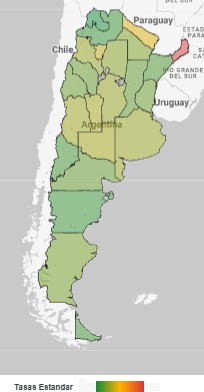
\includegraphics{mapa_tasas.jpeg} En el mapa también vemos que la única
provincia con tasa muy alta es Misiones ya que aparece en color rojo.

\begin{Shaded}
\begin{Highlighting}[]
\FunctionTok{library}\NormalTok{(ggplot2)}

\NormalTok{tabla\_para\_mostrar2 }\OtherTok{\textless{}{-}}\NormalTok{ df\_resultados }\SpecialCharTok{\%\textgreater{}\%} \CommentTok{\# Usamos el df\_resultados ya transformado}
  \FunctionTok{select}\NormalTok{(}
    \AttributeTok{Provincia =}\NormalTok{ provincia,}
    \AttributeTok{RME =}\NormalTok{ rme}
\NormalTok{  ) }
\CommentTok{\# Mostrar la tabla usando kable}
\FunctionTok{kable}\NormalTok{(tabla\_para\_mostrar2, }\AttributeTok{caption =} \StringTok{"Tabla 2: Razones de Mortalidad Estandarizadas por Provincia"}\NormalTok{) }\SpecialCharTok{\%\textgreater{}\%}
  \FunctionTok{kable\_styling}\NormalTok{(}
    \AttributeTok{bootstrap\_options =} \FunctionTok{c}\NormalTok{(}\StringTok{"striped"}\NormalTok{, }\StringTok{"hover"}\NormalTok{, }\StringTok{"condensed"}\NormalTok{, }\StringTok{"responsive"}\NormalTok{), }\CommentTok{\# Opciones de estilo Bootstrap}
    \AttributeTok{full\_width =} \ConstantTok{FALSE}\NormalTok{, }\CommentTok{\# La tabla no ocupa todo el ancho de la página}
    \AttributeTok{position =} \StringTok{"left"}\NormalTok{) }\SpecialCharTok{\%\textgreater{}\%}  \CommentTok{\# Alinea la tabla a la izquierda}
    \FunctionTok{row\_spec}\NormalTok{(}\AttributeTok{row =} \DecValTok{0}\NormalTok{, }\AttributeTok{background =} \StringTok{"steelblue"}\NormalTok{, }\AttributeTok{color =} \StringTok{"black"}\NormalTok{, }\AttributeTok{extra\_css =} \StringTok{"font{-}weight: bold;"}\NormalTok{) }\SpecialCharTok{\%\textgreater{}\%} 
  \FunctionTok{row\_spec}\NormalTok{(}\AttributeTok{row =} \FunctionTok{c}\NormalTok{(}\DecValTok{2}\NormalTok{, }\DecValTok{9}\NormalTok{, }\DecValTok{11}\NormalTok{, }\DecValTok{13}\NormalTok{, }\DecValTok{14}\NormalTok{, }\DecValTok{19}\NormalTok{, }\DecValTok{24}\NormalTok{), }\AttributeTok{background =} \StringTok{"lightblue"}\NormalTok{, }\AttributeTok{color =} \StringTok{"black"}\NormalTok{)}
\end{Highlighting}
\end{Shaded}

\begin{longtable}[l]{lr}
\caption{\label{tab:unnamed-chunk-7}Tabla 2: Razones de Mortalidad Estandarizadas por Provincia}\\
\toprule
\cellcolor{steelblue}{\textcolor{black}{Provincia}} & \cellcolor{steelblue}{\textcolor{black}{RME}}\\
\midrule
Buenos Aires & 0.9938174\\
\cellcolor{lightblue}{\textcolor{black}{C.A.B.A.}} & \cellcolor{lightblue}{\textcolor{black}{1.5126843}}\\
Catamarca & 0.9915571\\
Chaco & 0.8772738\\
Chubut & 0.3848355\\
\addlinespace
Cordoba & 0.9931523\\
Corrientes & 0.5071060\\
Entre Rios & 0.6836319\\
\cellcolor{lightblue}{\textcolor{black}{Formosa}} & \cellcolor{lightblue}{\textcolor{black}{1.5334733}}\\
Jujuy & 0.1515395\\
\addlinespace
\cellcolor{lightblue}{\textcolor{black}{La Pampa}} & \cellcolor{lightblue}{\textcolor{black}{1.1036673}}\\
La Rioja & 0.6605521\\
\cellcolor{lightblue}{\textcolor{black}{Mendoza}} & \cellcolor{lightblue}{\textcolor{black}{1.0386637}}\\
\cellcolor{lightblue}{\textcolor{black}{Misiones}} & \cellcolor{lightblue}{\textcolor{black}{3.1635893}}\\
Neuquen & 0.4434360\\
\addlinespace
Rio Negro & 0.6472000\\
Salta & 0.3894801\\
San Juan & 0.6815738\\
\cellcolor{lightblue}{\textcolor{black}{San Luis}} & \cellcolor{lightblue}{\textcolor{black}{1.1162325}}\\
Santa Cruz & 0.8910036\\
\addlinespace
Sante Fe & 0.6282376\\
Santiago del Estero & 0.8811364\\
Tierra Del Fuego & 0.4833651\\
\cellcolor{lightblue}{\textcolor{black}{Tucuman}} & \cellcolor{lightblue}{\textcolor{black}{1.3173715}}\\
\bottomrule
\end{longtable}

\begin{Shaded}
\begin{Highlighting}[]
\FunctionTok{ggplot}\NormalTok{(df\_resultados) }\SpecialCharTok{+} \CommentTok{\# Assuming your dataframe is named df\_resultados\_consolidados}
  \FunctionTok{aes}\NormalTok{(}\AttributeTok{x =}\NormalTok{ provincia, }\AttributeTok{y =}\NormalTok{ rme) }\SpecialCharTok{+}
  \FunctionTok{geom\_col}\NormalTok{(}\AttributeTok{fill =} \StringTok{"steelblue"}\NormalTok{) }\SpecialCharTok{+} \CommentTok{\# Use geom\_col() for pre{-}summarized data}
  \FunctionTok{labs}\NormalTok{(}
    \AttributeTok{title =} \StringTok{"Razón de Mortalidad Estandarizada (RME) por Provincia"}\NormalTok{,}
    \AttributeTok{x =} \StringTok{"Provincia"}\NormalTok{,}
    \AttributeTok{y =} \StringTok{"RME"}
\NormalTok{  ) }\SpecialCharTok{+}
  \FunctionTok{geom\_hline}\NormalTok{(}\AttributeTok{yintercept =} \DecValTok{1}\NormalTok{, }\AttributeTok{linetype =} \StringTok{"dashed"}\NormalTok{, }\AttributeTok{color =} \StringTok{"red"}\NormalTok{, }\AttributeTok{linewidth =} \FloatTok{0.8}\NormalTok{) }\SpecialCharTok{+}
  \FunctionTok{theme\_minimal}\NormalTok{() }\SpecialCharTok{+} \CommentTok{\# A cleaner theme}
  \FunctionTok{theme}\NormalTok{(}\AttributeTok{axis.text.x =} \FunctionTok{element\_text}\NormalTok{(}\AttributeTok{angle =} \DecValTok{45}\NormalTok{, }\AttributeTok{hjust =} \DecValTok{1}\NormalTok{))}
\end{Highlighting}
\end{Shaded}

\includegraphics{reporte_tp3_files/figure-latex/unnamed-chunk-7-1.pdf}

Una vez calculadas las razones de mortalidad estandarizadas para cada
provincia por el método indirecto vemos que

Razón de Mortalidad Estandarizada (RME) por Provincia en Argentina
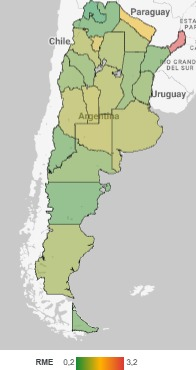
\includegraphics{map_rme.jpeg}

\end{document}
